% This LaTeX document needs to be compiled with XeLaTeX.
\documentclass[10pt]{article}
\usepackage[utf8]{inputenc}
\usepackage{graphicx}
\usepackage[export]{adjustbox}
\graphicspath{ {./images/} }
\usepackage{amsmath}
\usepackage{amsfonts}
\usepackage{amssymb}
\usepackage[version=4]{mhchem}
\usepackage{stmaryrd}
\usepackage[fallback]{xeCJK}
\usepackage{polyglossia}
\usepackage{fontspec}
\setCJKmainfont{Noto Serif CJK JP}

\setmainlanguage{polish}
\setmainfont{CMU Serif}

\title{Egzamin maturalny }

\author{}
\date{}


\begin{document}
\maketitle
KOD

\begin{center}
\begin{tabular}{|l|l|l|l|l|l|l|l|l|l|}
\hline
 &  &  \\
\hline
 &  &  \\
\hline
\end{tabular}
\end{center}

\section*{Miejsce na naklejkę.}
Sprawdż, czy kod na naklejce to M-100.

Jeżeli tak - przyklej naklejkę. Jeżeli nie - zgłoś to nauczycielowi.

\section*{Formuła 2023}
\section*{MATEMATYKA}
\section*{Poziom rozszerzony}
Symbol arkusza\\
MMAP-RO-100-2305

\section*{Data: 12 maja 2023 r. \\
 GODZINA ROZPOCZECIA: 9:00}
WYPEとNIA ZESPÓŁ NADZORUJĄCY\\
Uprawnienia zdającego do:\\
dostosowania zasad oceniania\\
CZAS tRWANIA: 180 minut\\
dostosowania w zw. z dyskalkulią.

LICZBA PUNKTÓW DO UZYSKANIA: 50

Przed rozpoczęciem pracy z arkuszem egzaminacyjnym

\begin{enumerate}
  \item Sprawdź, czy nauczyciel przekazał Ci właściwy arkusz egzaminacyjny, tj. arkusz we właściwej formule, z właściwego przedmiotu na właściwym poziomie.
  \item Jeżeli przekazano Ci niewłaściwy arkusz - natychmiast zgłoś to nauczycielowi. Nie rozrywaj banderol.
  \item Jeżeli przekazano Ci właściwy arkusz - rozerwij banderole po otrzymaniu takiego polecenia od nauczyciela. Zapoznaj się z instrukcją na stronie 2.\\

\includegraphics[max width=\textwidth, center]{2024_11_21_f1ecc00f5c4ab21f0d04g-01}\\

\includegraphics[max width=\textwidth, center]{2024_11_21_f1ecc00f5c4ab21f0d04g-02}
\end{enumerate}

\section*{Instrukcja dla zdającego}
\begin{enumerate}
  \item Sprawdź, czy arkusz egzaminacyjny zawiera 27 stron (zadania 1-13). Ewentualny brak zgłoś przewodniczącemu zespołu nadzorującego egzamin.
  \item Na pierwszej stronie arkusza oraz na karcie odpowiedzi wpisz swój numer PESEL i przyklej naklejkę z kodem.
  \item Pamiętaj, że pominięcie argumentacji lub istotnych obliczeń w rozwiązaniu zadania otwartego może spowodować, że za to rozwiązanie nie otrzymasz pełnej liczby punktów.
  \item Rozwiązania zadań i odpowiedzi wpisuj w miejscu na to przeznaczonym.
  \item Pisz czytelnie i używaj tylko długopisu lub pióra z czarnym tuszem lub atramentem.
  \item Nie używaj korektora, a błędne zapisy wyraźnie przekreśl.
  \item Nie wpisuj żadnych znaków w tabelkach przeznaczonych dla egzaminatora. Tabelki umieszczone są na marginesie przy każdym zadaniu.
  \item Pamiętaj, że zapisy w brudnopisie nie będą oceniane.
  \item Możesz korzystać z Wybranych wzorów matematycznych, cyrkla i linijki oraz kalkulatora prostego. Upewnij się, czy przekazano Ci broszurę z okładką taką jak widoczna poniżej.\\
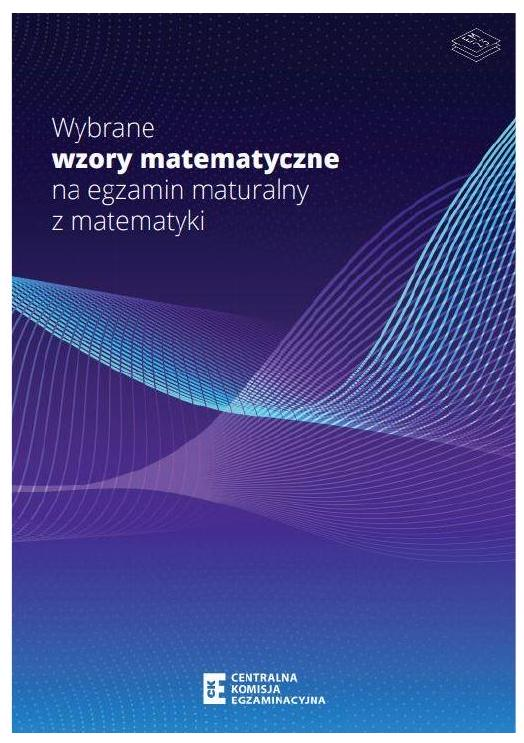
\includegraphics[max width=\textwidth, center]{2024_11_21_f1ecc00f5c4ab21f0d04g-02(1)}
\end{enumerate}

\section*{Zadania egzaminacyjne są wydrukowane na następnych stronach.}
\section*{Zadanie 1. (0-2)}
W chwili początkowej \((t=0)\) masa substancji jest równa 4 gramom. Wskutek rozpadu cząsteczek tej substancji jej masa się zmniejsza. Po każdej kolejnej dobie ubywa \(19 \%\) masy, jaka była na koniec doby poprzedniej. Dla każdej liczby całkowitej \(t \geq 0\) funkcja \(m(t)\) określa masę substancji w gramach po \(t\) pełnych dobach (czas liczymy od chwili początkowej).

Wyznacz wzór funkcji \(\boldsymbol{m}(t)\). Oblicz, po ilu pełnych dobach masa tej substancji będzie po raz pierwszy mniejsza od 1,5 grama.\\
Zapisz obliczenia.\\

\includegraphics[max width=\textwidth, center]{2024_11_21_f1ecc00f5c4ab21f0d04g-04}

Zadanie 2. (0-3)\\
Tomek i Romek postanowili rozegrać między sobą pięć partii szachów. Prawdopodobieństwo wygrania pojedynczej partii przez Tomka jest równe \(\frac{1}{4}\).

Oblicz prawdopodobieństwo wygrania przez Tomka co najmniej czterech z pięciu partii. Wynik podaj w postaci ułamka zwykłego nieskracalnego. Zapisz obliczenia.\\

\includegraphics[max width=\textwidth, center]{2024_11_21_f1ecc00f5c4ab21f0d04g-05}

Zadanie 3. (0-3)\\
Funkcja \(f\) jest określona wzorem \(f(x)=\frac{3 x^{2}-2 x}{x^{2}+2 x+8}\) dla każdej liczby rzeczywistej \(x\). Punkt \(P=\left(x_{0}, 3\right)\) należy do wykresu funkcji \(f\).

Oblicz \(x_{0}\) oraz wyznacz równanie stycznej do wykresu funkcji \(f\) w punkcie \(P\). Zapisz obliczenia.\\

\includegraphics[max width=\textwidth, center]{2024_11_21_f1ecc00f5c4ab21f0d04g-06}

Zadanie 4. (0-3)\\
Liczby rzeczywiste \(x\) oraz \(y\) spełniają jednocześnie równanie \(x+y=4\) i nierówność \(x^{3}-x^{2} y \leq x y^{2}-y^{3}\).

Wykaż, że \(x=2\) oraz \(y=2\).\\

\includegraphics[max width=\textwidth, center]{2024_11_21_f1ecc00f5c4ab21f0d04g-07}

Zadanie 5. (0-3)\\
Dany jest trójkąt prostokątny \(A B C\), w którym \(|\measuredangle A B C|=90^{\circ}\) oraz \(|\measuredangle C A B|=60^{\circ}\). Punkty \(K\) i \(L\) leżą na bokach - odpowiednio \(-A B\) i \(B C\) tak, że \(|B K|=|B L|=1\) (zobacz rysunek). Odcinek \(K L\) przecina wysokość \(B D\) tego trójkąta w punkcie \(N\), a ponadto \(|A D|=2\).\\
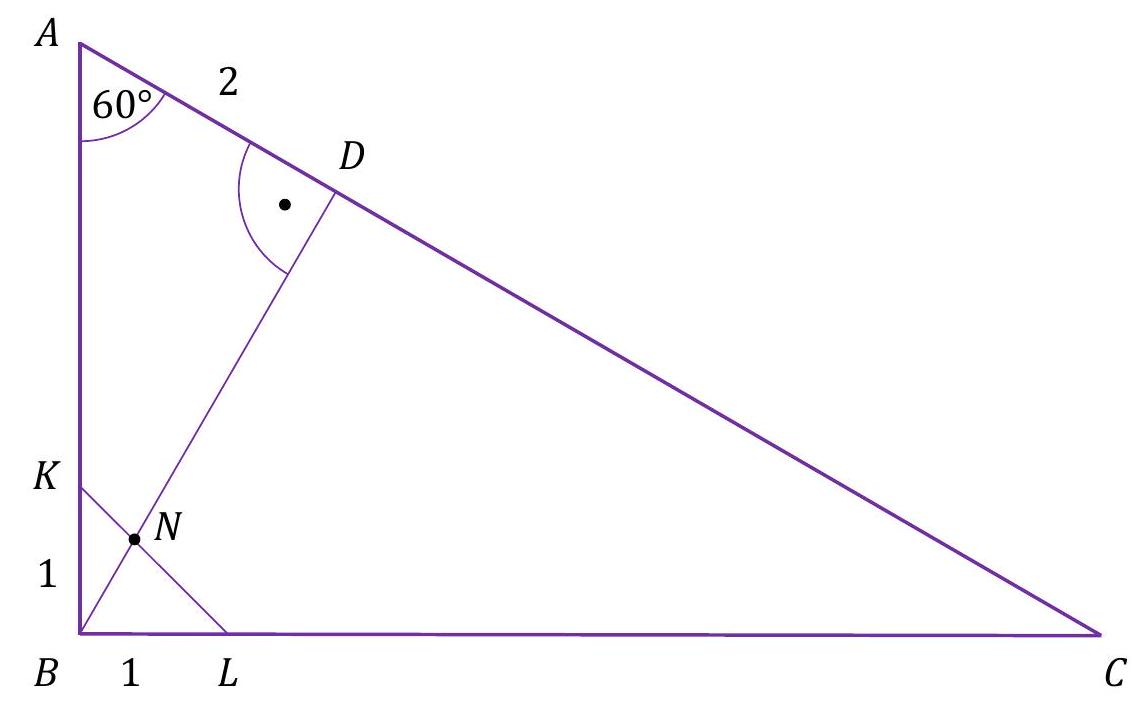
\includegraphics[max width=\textwidth, center]{2024_11_21_f1ecc00f5c4ab21f0d04g-08(1)}

Wykaż, że \(|N D|=\sqrt{3}+1\).

\begin{center}
\begin{tabular}{|c|c|c|c|c|c|c|c|c|c|c|c|c|c|c|c|c|c|c|c|c|c|c|c|c|c|c|c|c|c|}
\hline
 &  &  &  &  &  &  &  &  &  &  &  &  &  &  &  &  &  &  &  &  &  &  &  &  &  &  &  &  &  \\
\hline
 &  &  &  &  &  &  &  &  &  &  &  &  &  &  &  &  &  &  &  &  &  &  &  &  &  &  &  &  &  \\
\hline
 &  &  &  &  &  &  &  &  &  &  &  &  &  &  &  &  &  &  &  &  &  &  &  &  &  &  &  &  &  \\
\hline
 &  &  &  &  &  &  &  &  &  &  &  &  &  &  &  &  &  &  &  &  &  &  &  &  &  &  &  &  &  \\
\hline
 &  &  &  &  &  &  &  &  &  &  &  &  &  &  &  &  &  &  &  &  &  &  &  &  &  &  &  &  &  \\
\hline
 &  &  &  &  &  &  &  &  &  &  &  &  &  &  &  &  &  &  &  &  &  &  &  &  &  &  &  &  &  \\
\hline
 &  &  &  &  &  &  &  &  &  &  &  &  &  &  &  &  &  &  &  &  &  &  &  &  &  &  &  &  &  \\
\hline
 &  &  &  &  &  &  &  &  &  &  &  &  &  &  &  &  &  &  &  &  &  &  &  &  &  &  &  &  &  \\
\hline
 &  &  &  &  &  &  &  &  &  &  &  &  &  &  &  &  &  &  &  &  &  &  &  &  &  &  &  &  &  \\
\hline
 &  &  &  &  &  &  &  &  &  &  &  &  &  &  &  &  &  &  &  &  &  &  &  &  &  &  &  &  &  \\
\hline
 &  &  &  &  &  &  &  &  &  &  &  &  &  &  &  &  &  &  &  &  &  &  &  &  &  &  &  &  &  \\
\hline
 &  &  &  &  &  &  &  &  &  &  &  &  &  &  &  &  &  &  &  &  &  &  &  &  &  &  &  &  &  \\
\hline
 &  &  &  &  &  &  &  &  &  &  &  &  &  &  &  &  &  &  &  &  &  &  &  &  &  &  &  &  &  \\
\hline
 &  &  &  &  &  &  &  &  &  &  &  &  &  &  &  &  &  &  &  &  &  &  &  &  &  &  &  &  &  \\
\hline
 &  &  &  &  &  &  &  &  &  &  &  &  &  &  &  &  &  &  &  &  &  &  &  &  &  &  &  &  &  \\
\hline
 &  &  &  &  &  &  &  &  &  &  &  &  &  &  &  &  &  &  &  &  &  &  &  &  &  &  &  &  &  \\
\hline
 &  &  &  &  &  &  &  &  &  &  &  &  &  &  &  &  &  &  &  &  &  &  &  &  &  &  &  &  &  \\
\hline
 &  &  &  &  &  &  &  &  &  &  &  &  &  &  &  &  &  &  &  &  &  &  &  &  &  &  &  &  &  \\
\hline
 &  &  &  &  &  &  &  &  &  &  &  &  &  &  &  &  &  &  &  &  &  &  &  &  &  &  &  &  &  \\
\hline
 &  &  &  &  &  &  &  &  &  &  &  &  &  &  &  &  &  &  &  &  &  &  &  &  &  &  &  &  &  \\
\hline
 &  &  &  &  &  &  &  &  &  &  &  &  &  &  &  &  &  &  &  &  &  &  &  &  &  &  &  &  &  \\
\hline
 &  &  &  &  &  &  &  &  &  &  &  &  &  &  &  &  &  &  &  &  &  &  &  &  &  & 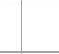
\includegraphics[max width=\textwidth]{2024_11_21_f1ecc00f5c4ab21f0d04g-08}
 &  &  &  \\
\hline
 &  &  &  &  &  &  &  &  &  &  &  &  &  &  &  &  &  &  &  &  &  &  &  &  &  &  &  &  &  \\
\hline
 &  &  &  &  &  &  &  &  &  &  &  &  &  &  &  &  &  &  &  &  &  &  &  &  &  &  &  &  &  \\
\hline
\end{tabular}
\end{center}

\begin{center}

\includegraphics[max width=\textwidth]{2024_11_21_f1ecc00f5c4ab21f0d04g-09}
\end{center}

\[
4 \sin (4 x) \cos (6 x)=2 \sin (10 x)+1
\]

\section*{Zapisz obliczenia.}
\begin{center}

\includegraphics[max width=\textwidth]{2024_11_21_f1ecc00f5c4ab21f0d04g-10}
\end{center}

Zadanie 7. (0-4)\\
Dany jest sześcian ABCDEFGH o krawędzi długości 6. Punkt \(S\) jest punktem przecięcia przekątnych \(A H\) i \(D E\) ściany bocznej \(A D H E\) (zobacz rysunek).\\
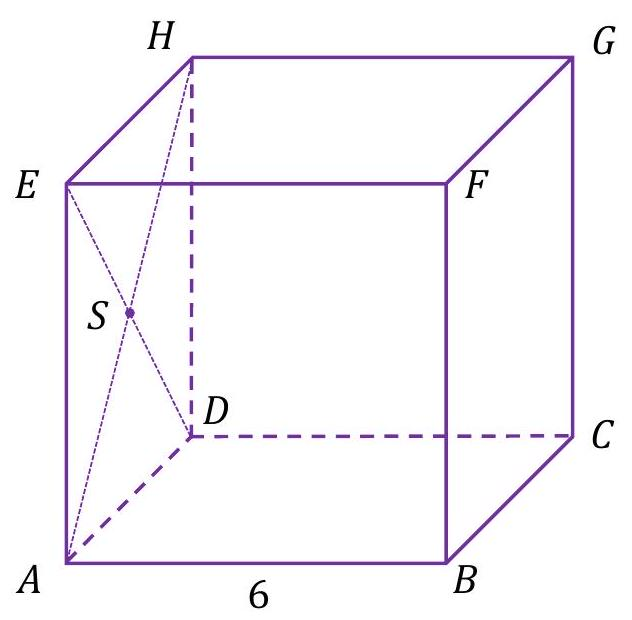
\includegraphics[max width=\textwidth, center]{2024_11_21_f1ecc00f5c4ab21f0d04g-11}

Oblicz wysokość trójkąta SBH poprowadzoną z punktu \(S\) na bok \(B H\) tego trójkąta. Zapisz obliczenia.\\

\includegraphics[max width=\textwidth, center]{2024_11_21_f1ecc00f5c4ab21f0d04g-11(1)}

Zadanie 8. (0-4)\\
Czworokąt \(A B C D\), w którym \(|B C|=4\) i \(|C D|=5\), jest opisany na okręgu. Przekątna \(A C\) tego czworokąta tworzy z bokiem \(B C\) kąt o mierze \(60^{\circ}\), natomiast z bokiem \(A B\)-kąt ostry, którego sinus jest równy \(\frac{1}{4}\).

Oblicz obwód czworokąta \(A B C D\). Zapisz obliczenia.\\

\includegraphics[max width=\textwidth, center]{2024_11_21_f1ecc00f5c4ab21f0d04g-12}\\

\includegraphics[max width=\textwidth, center]{2024_11_21_f1ecc00f5c4ab21f0d04g-13}

Zadanie 9. (0-4)\\
Rozwiąż nierówność

\[
\sqrt{x^{2}+4 x+4}<\frac{25}{3}-\sqrt{x^{2}-6 x+9}
\]

Zapisz obliczenia.\\
Wskazówka: skorzystaj z tego, że \(\sqrt{a^{2}}=|a|\) dla każdej liczby rzeczywistej \(a\).

\begin{center}
\begin{tabular}{|c|c|c|c|c|c|c|c|c|c|c|c|c|c|c|c|c|c|c|c|c|c|c|c|c|}
\hline
 &  &  &  &  &  &  &  &  &  &  &  &  &  &  &  &  &  &  &  &  &  &  &  &  \\
\hline
 &  &  &  &  &  &  &  &  &  &  &  &  &  &  &  &  &  &  &  &  &  &  &  &  \\
\hline
 &  &  &  &  &  &  &  &  &  &  &  &  &  &  &  &  &  &  &  &  &  &  &  &  \\
\hline
 &  &  &  &  &  &  &  &  &  &  &  &  &  &  &  &  &  &  &  &  &  &  &  &  \\
\hline
 &  &  &  &  &  &  &  &  &  &  &  &  &  &  &  &  &  &  &  &  &  &  &  &  \\
\hline
 &  &  &  &  &  &  &  &  &  &  &  &  &  &  &  &  &  &  &  &  &  &  &  &  \\
\hline
 &  &  &  &  &  &  &  &  &  &  &  &  &  &  &  &  &  &  &  &  &  &  &  &  \\
\hline
 &  &  &  &  &  &  &  &  &  &  &  &  &  &  &  &  &  &  &  &  &  &  &  &  \\
\hline
 &  &  &  &  &  &  &  &  &  &  &  &  &  &  &  &  &  &  &  &  &  &  &  &  \\
\hline
 &  &  &  &  &  &  &  &  &  &  &  &  &  &  &  &  &  &  &  &  &  &  &  &  \\
\hline
 &  &  &  &  &  &  &  &  &  &  &  &  &  &  &  &  &  &  &  &  &  &  &  &  \\
\hline
 &  &  &  &  &  &  &  &  &  &  &  &  &  &  &  &  &  &  &  &  &  &  &  &  \\
\hline
 &  &  &  &  &  &  &  &  &  &  &  &  &  &  &  &  &  &  &  &  &  &  &  &  \\
\hline
 &  &  &  &  &  &  &  &  &  &  &  &  &  &  &  &  &  &  &  &  &  &  &  &  \\
\hline
 &  &  &  &  &  &  &  &  &  &  &  &  &  &  &  &  &  &  &  &  &  &  &  &  \\
\hline
 &  &  &  &  &  &  &  &  &  &  &  &  &  &  &  &  &  &  &  &  &  &  &  &  \\
\hline
 &  &  &  &  &  &  &  &  &  &  &  &  &  &  &  &  &  &  &  &  &  &  &  &  \\
\hline
 &  &  &  &  &  &  &  &  &  &  &  &  &  &  &  &  &  &  &  &  &  &  &  &  \\
\hline
 &  &  &  &  &  &  &  &  &  &  &  &  &  &  &  &  &  &  &  &  &  &  &  &  \\
\hline
 &  &  &  &  &  &  &  &  &  &  &  &  &  &  &  &  &  &  &  &  &  &  &  &  \\
\hline
 &  &  &  &  &  &  &  &  &  &  &  &  &  &  &  &  &  &  &  &  &  &  &  &  \\
\hline
 &  &  &  &  &  &  &  &  &  &  &  &  &  &  &  &  &  &  &  &  &  &  &  &  \\
\hline
 &  &  &  &  &  &  &  &  &  &  &  &  &  &  &  &  &  &  &  &  &  &  &  &  \\
\hline
 &  &  &  &  &  &  &  &  &  &  &  &  &  &  &  &  &  &  &  &  &  &  &  &  \\
\hline
 &  &  &  &  &  &  &  &  &  &  &  &  &  &  &  &  &  &  &  &  &  &  &  &  \\
\hline
 &  &  &  &  &  &  &  &  &  &  &  &  &  &  &  &  &  &  &  &  &  &  &  &  \\
\hline
 &  &  &  &  &  &  &  &  &  &  &  &  &  &  &  &  &  &  &  &  &  &  &  &  \\
\hline
 &  &  &  &  &  &  &  &  &  &  &  &  &  &  &  &  &  &  &  &  &  &  &  &  \\
\hline
 &  &  &  &  &  &  &  &  &  &  &  &  &  &  &  &  &  &  &  &  &  &  &  &  \\
\hline
 &  &  &  &  &  &  &  &  &  &  &  &  &  &  &  &  &  &  &  &  &  &  &  &  \\
\hline
 &  &  &  &  &  &  &  &  &  &  &  &  &  &  &  &  &  &  &  &  &  &  &  &  \\
\hline
 &  &  &  &  &  &  &  &  &  &  &  &  &  &  &  &  &  &  &  &  &  &  &  &  \\
\hline
 &  &  &  &  &  &  &  &  &  &  &  &  &  &  &  &  &  &  &  &  &  &  &  &  \\
\hline
 &  &  &  &  &  &  &  &  &  &  &  &  &  &  &  &  &  &  &  &  &  &  &  &  \\
\hline
 &  &  &  &  &  &  &  &  &  &  &  &  &  &  &  &  &  &  &  &  &  &  &  &  \\
\hline
 &  &  &  &  &  &  &  &  &  &  &  &  &  &  &  &  &  &  &  &  &  &  &  &  \\
\hline
 &  &  &  &  &  &  &  &  &  &  &  &  &  &  &  &  &  &  &  &  &  &  &  &  \\
\hline
 &  &  &  &  &  &  &  &  &  &  &  &  &  &  &  &  &  &  &  &  &  &  &  &  \\
\hline
\end{tabular}
\end{center}

\begin{center}

\includegraphics[max width=\textwidth]{2024_11_21_f1ecc00f5c4ab21f0d04g-15}
\end{center}

Zadanie 10. (0-4)\\
Określamy kwadraty \(K_{1}, K_{2}, K_{3}, \ldots\) następująco:

\begin{itemize}
  \item \(K_{1}\) jest kwadratem o boku długości \(a\)
  \item \(K_{2}\) jest kwadratem, którego każdy wierzchołek leży na innym boku kwadratu \(K_{1}\) i dzieli ten bok w stosunku 1:3
  \item \(K_{3}\) jest kwadratem, którego każdy wierzchołek leży na innym boku kwadratu \(K_{2}\) i dzieli ten bok w stosunku 1:3\\
i ogólnie, dla każdej liczby naturalnej \(n \geq 2\),
  \item \(K_{n}\) jest kwadratem, którego każdy wierzchołek leży na innym boku kwadratu \(K_{n-1}\) i dzieli ten bok w stosunku 1:3.\\
Obwody wszystkich kwadratów określonych powyżej tworzą nieskończony ciąg geometryczny.\\
Na rysunku przedstawiono kwadraty utworzone w sposób opisany powyżej.\\
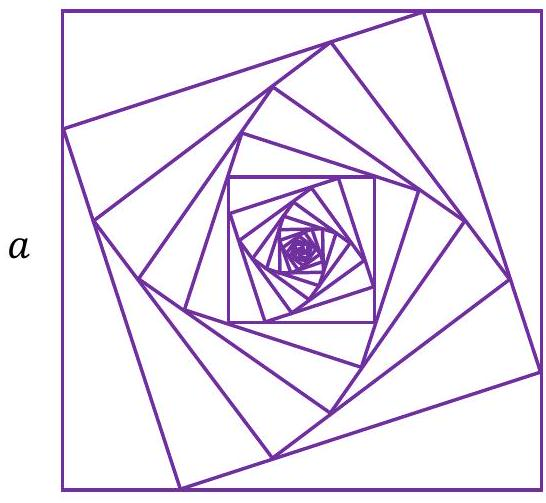
\includegraphics[max width=\textwidth, center]{2024_11_21_f1ecc00f5c4ab21f0d04g-16(2)}\\
a\\
Oblicz sumę wszystkich wyrazów tego nieskończonego ciągu. Zapisz obliczenia.
\end{itemize}

\begin{center}
\begin{tabular}{|c|c|c|c|c|c|c|c|c|c|c|c|c|c|c|c|c|c|c|c|c|c|c|c|c|c|c|c|c|}
\hline
 &  &  &  &  &  &  &  &  &  &  &  &  &  &  &  &  &  &  &  &  &  &  &  &  &  &  &  &  \\
\hline
 &  &  &  &  &  &  &  &  &  &  &  &  &  &  &  &  &  &  &  &  &  &  &  &  &  &  &  &  \\
\hline
 &  &  &  &  &  &  &  &  &  &  &  &  &  &  &  &  &  &  &  &  &  &  &  &  &  &  &  &  \\
\hline
 &  &  &  &  &  &  &  &  &  &  &  &  &  &  &  &  &  &  &  &  &  &  &  &  &  &  &  &  \\
\hline
 &  &  &  &  &  &  &  &  &  &  &  &  &  &  &  &  &  &  &  &  &  &  &  &  &  &  &  &  \\
\hline
 &  &  &  &  &  &  &  &  &  &  &  &  &  &  &  &  &  &  &  &  &  &  &  &  &  &  &  &  \\
\hline
 &  &  &  &  &  &  &  &  &  &  &  &  &  &  &  &  &  &  &  &  &  &  &  &  &  &  &  &  \\
\hline
 &  &  &  &  &  &  &  &  &  &  &  &  &  &  &  &  &  &  &  &  &  &  &  &  &  &  &  &  \\
\hline
 &  &  &  &  &  &  &  &  &  &  &  &  &  &  &  &  &  &  &  &  &  &  &  &  &  &  &  &  \\
\hline
 &  &  &  &  &  &  &  &  &  &  &  &  &  &  &  &  &  &  &  &  &  &  &  &  &  &  &  &  \\
\hline
 &  &  &  &  &  &  &  &  &  &  &  &  &  &  &  &  &  &  &  &  &  &  &  &  &  &  &  &  \\
\hline
 &  &  &  &  &  &  &  &  &  &  &  &  &  &  &  &  &  &  &  &  &  &  &  &  & , &  &  &  \\
\hline
 &  &  &  &  &  &  &  &  &  &  &  &  &  &  &  &  &  &  &  &  &  &  &  &  &  &  &  &  \\
\hline
 &  &  &  &  &  &  &  &  &  &  &  &  &  &  &  &  &  &  &  &  &  &  &  &  &  &  &  &  \\
\hline
 &  &  &  &  &  &  &  &  &  &  &  &  &  &  &  &  &  &  &  &  &  &  &  &  &  &  &  &  \\
\hline
 &  &  &  &  &  &  &  &  &  &  &  &  &  &  &  &  &  &  &  &  &  &  &  &  &  &  &  &  \\
\hline
 &  &  &  &  &  &  &  &  &  &  &  &  &  &  &  &  &  &  &  &  &  &  &  &  &  &  &  &  \\
\hline
 &  &  &  &  &  &  &  &  &  &  &  &  &  &  &  &  &  &  &  &  &  & 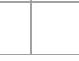
\includegraphics[max width=\textwidth]{2024_11_21_f1ecc00f5c4ab21f0d04g-16(1)}
 &  &  & 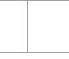
\includegraphics[max width=\textwidth]{2024_11_21_f1ecc00f5c4ab21f0d04g-16}
 &  &  &  \\
\hline
\end{tabular}
\end{center}

\begin{center}

\includegraphics[max width=\textwidth]{2024_11_21_f1ecc00f5c4ab21f0d04g-17}
\end{center}

Zadanie 11. (0-5)\\
Wyznacz wszystkie wartości parametru \(\boldsymbol{m} \neq \mathbf{2}\), dla których równanie

\[
x^{2}+4 x-\frac{m-3}{m-2}=0
\]

ma dwa różne rozwiązania rzeczywiste \(x_{1}, x_{2}\) spełniające warunek \(x_{1}^{3}+x_{2}^{3}>-28\). Zapisz obliczenia.\\

\includegraphics[max width=\textwidth, center]{2024_11_21_f1ecc00f5c4ab21f0d04g-18}\\

\includegraphics[max width=\textwidth, center]{2024_11_21_f1ecc00f5c4ab21f0d04g-19}

\section*{Zadanie 12.}
Funkcja \(f\) jest określona wzorem \(f(x)=81^{\log _{3} x}+\frac{2 \cdot \log _{2} \sqrt{27} \cdot \log _{3} 2}{3} \cdot x^{2}-6 x\) dla każdej liczby dodatniej \(x\).

Zadanie 12.1. (0-2)\\
Wykaż, że dla każdej liczby dodatniej \(x\) wyrażenie

\[
81^{\log _{3} x}+\frac{2 \cdot \log _{2} \sqrt{27} \cdot \log _{3} 2}{3} \cdot x^{2}-6 x
\]

można równoważnie przekształcić do postaci \(x^{4}+x^{2}-6 x\).\\

\includegraphics[max width=\textwidth, center]{2024_11_21_f1ecc00f5c4ab21f0d04g-20}

Zadanie 12.2. (0-4)\\
Oblicz najmniejszą wartość funkcji \(f\) określonej dla każdej liczby dodatniej \(x\). Zapisz obliczenia.

Wskazówka: przyjmij, że wzór funkcji \(f\) można przedstawić w postaci \(f(x)=x^{4}+x^{2}-6 x\).\\
\(\qquad\)

Zadanie 13. (0-6)\\
W kartezjańskim układzie współrzędnych \((x, y)\) prosta \(l\) o równaniu \(x-y-2=0\) przecina parabolę o równaniu \(y=4 x^{2}-7 x+1\) w punktach \(A\) oraz \(B\). Odcinek \(A B\) jest średnicą okręgu \(\mathcal{O}\). Punkt \(C\) leży na okręgu \(\mathcal{O}\) nad prostą \(l\), a kąt \(B A C\) jest ostry i ma miarę \(\alpha\) taką, że \(\operatorname{tg} \alpha=\frac{1}{3}\) (zobacz rysunek).\\
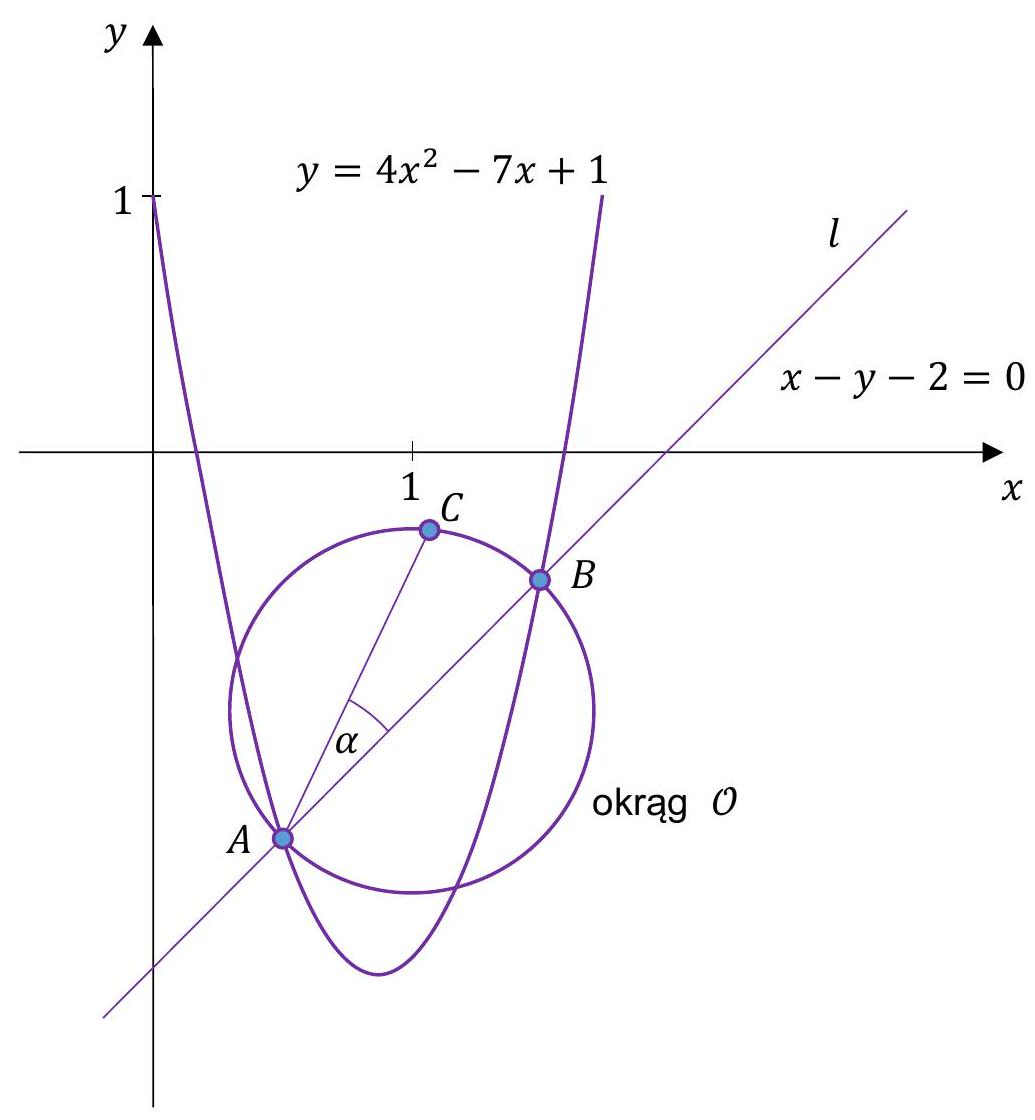
\includegraphics[max width=\textwidth, center]{2024_11_21_f1ecc00f5c4ab21f0d04g-22(1)}

Oblicz współrzędne punktu C. Zapisz obliczenia.\\

\includegraphics[max width=\textwidth, center]{2024_11_21_f1ecc00f5c4ab21f0d04g-22}\\

\includegraphics[max width=\textwidth, center]{2024_11_21_f1ecc00f5c4ab21f0d04g-23}\\

\includegraphics[max width=\textwidth, center]{2024_11_21_f1ecc00f5c4ab21f0d04g-24}

\section*{BRUDNOPIS (nie podlega ocenie)}

\includegraphics[max width=\textwidth, center]{2024_11_21_f1ecc00f5c4ab21f0d04g-25}\\

\includegraphics[max width=\textwidth, center]{2024_11_21_f1ecc00f5c4ab21f0d04g-26}\\

\includegraphics[max width=\textwidth, center]{2024_11_21_f1ecc00f5c4ab21f0d04g-27}

\section*{MATEMATYKA}
\section*{Poziom rozszerzony}
Formuła 2023

\section*{MATEMATYKA}
\section*{Poziom rozszerzony}
Formuła 2023

\section*{MATEMATYKA}
\section*{Poziom rozszerzony}
Formuła 2023


\end{document}